\chapter{Experimente}
\label{ch:experimente}

Die verwendeten Metriken der Experimente setzen sich zusammen aus Präzision (precision), Erinnerung (recall), F1-Wert (F1-Score) und Genauigkeit (accuracy). Zum Berechnen dieser wird das Vorkommen der Richtig-Positiven (TP), Falsch-Positiven (FP), Falsch-Negativen (FN) und Richtig-Negativen (TN) Vorhersagen des Modells benutzt. Die Kategorie TP zeigt vom Modell richtig erkannte Objekte, welche tatsächlich vorhanden sind, FP bestimmt die falsche Erkennung des Modells von Objekten, die in Wirklichkeit nicht vorhanden sind, FN gibt Auskunft über Objekte, die in der Realität vorhanden sind, das Modell sie allerdings nicht erkannt hat, und TN beschreibt Objekte, die korrekt als nicht vorhanden erkannt wurden.

\[Precision = \frac{TP}{TP + FP}\]

Precision misst den Anteil der korrekten positiven Vorhersagen an allen positiven Vorhersagen des Modells. Sie zeigt, wie genau das Modell bei der Erkennung von Objekten ist und wie gut es falsche positive Ergebnisse vermeidet. Ein hoher Precision-Wert bedeutet, dass wenn das Modell ein Objekt erkennt, es mit hoher Wahrscheinlichkeit tatsächlich vorhanden ist.

\[Recall = \frac{TP}{TP + FN}\]

Recall misst den Anteil der korrekt erkannten positiven Instanzen an allen tatsächlichen positiven Instanzen. Es zeigt, wie gut das Modell alle vorhandenen Objekte einer Klasse findet. Ein hoher Recall-Wert bedeutet, dass das Modell die meisten der tatsächlich vorhandenen Objekte erkennt.

\[F1 = 2 \cdot \frac{Precision \cdot Recall}{Precision + Recall}\]

Der F1-Wert ist das harmonische Mittel aus Precision und Recall. Ein hoher F1-Wert deutet darauf hin, dass das Modell sowohl präzise als auch umfassend in seinen Vorhersagen ist. Der F1-Wert ist besonders nützlich, wenn ein ausgewogenes Verhältnis zwischen Precision und Recall wichtig ist.

\[Accuracy = \frac{TP + TN}{TP + TN + FP + FN}\]

Die Richtigkeit (Accuracy) misst den Anteil aller korrekten Vorhersagen an der Gesamtzahl der Vorhersagen. Sie gibt nur an, wie oft das Modell insgesamt richtig liegt, weshalb sie nur bei der Klassifizierung verwendet wurde.
\\
Zum Visualisieren der Konfusionsmatrizen in diesem Kapitel wurde eine Kombination von \cite{2020SciPy-NMeth, DamianoP2024confusionMatrixGenerator} verwendet.

\section{Objekterkennung}

Für das Unterkapitel der Objekterkennung wurde die Effizienz, verschiedene Diagrammarten aus Texten mithilfe der Ultralytics YOLO Objekterkennungsmodelle zu extrahieren, untersucht. Hierfür wurden die erstellten Datensätze aus \ref{ch:chartbank} zum Vortrainieren und aus \ref{ch:scanbank} zum Feintrainieren verwendet.
\\
Ultralytics YOLO generiert nach abgeschlossenem Modelltraining automatisch verschiedene Metrikseinblicke. Insbesondere das eines F1-Confidence Diagramms. Aus diesem kann abgelesen werden, wie ein beliebiger Konfidenz-Schwellenwert (confidence threshold) der Modellvorhersagen die Evaluationsresultate des F1-Scores beeinflusst. Im Folgenden werden für alle Objekterkennungsexperimente jene Konfidenzwerte gewählt, welche den F1-Wert maximieren.

\subsection{Vortrainiertes Modell auf DocBank}
Um im Verlauf der Datensatzerstellung zu erforschen, ob die visuell ähnlichen Klassen der Balkendiagramme und Histogramme weiterhin differenziert werden sollen, wurde nach dem Erreichen einer Datensatzgröße von 200 Bildern der Datensatz mit Histogrammen sowie derselbe mit reduzierten Klassen evaluiert.

\subsection*{200 Trainingsbilder (mit Histogramme)}

Aufgrund der limitierten Anzahl an verfügbaren Validationsbildern bei einem so kleinen Datensatz können allerdings schwer überzeugende Aussagen getroffen werden.
Jedoch fällt die Verwechslung zwischen Balken und Histogramme in der Konfusionsmatrix trotzdem schnell auf. Grundsätzlich fallen die Evaluationswerte der Histogramm-Klasse vergleichsweise schlechter aus, weshalb im Weiteren die manuelle Annotation ohne Unterscheidung zwischen Histogrammen und Balkendiagrammen fortgeführt wurde.
\\
Die Evaluation wurde mit einem Confidence Threshold von 40.4\% durchgeführt.
\begin{figure}[H]
    \centering
    \captionsetup{width=1\linewidth}
    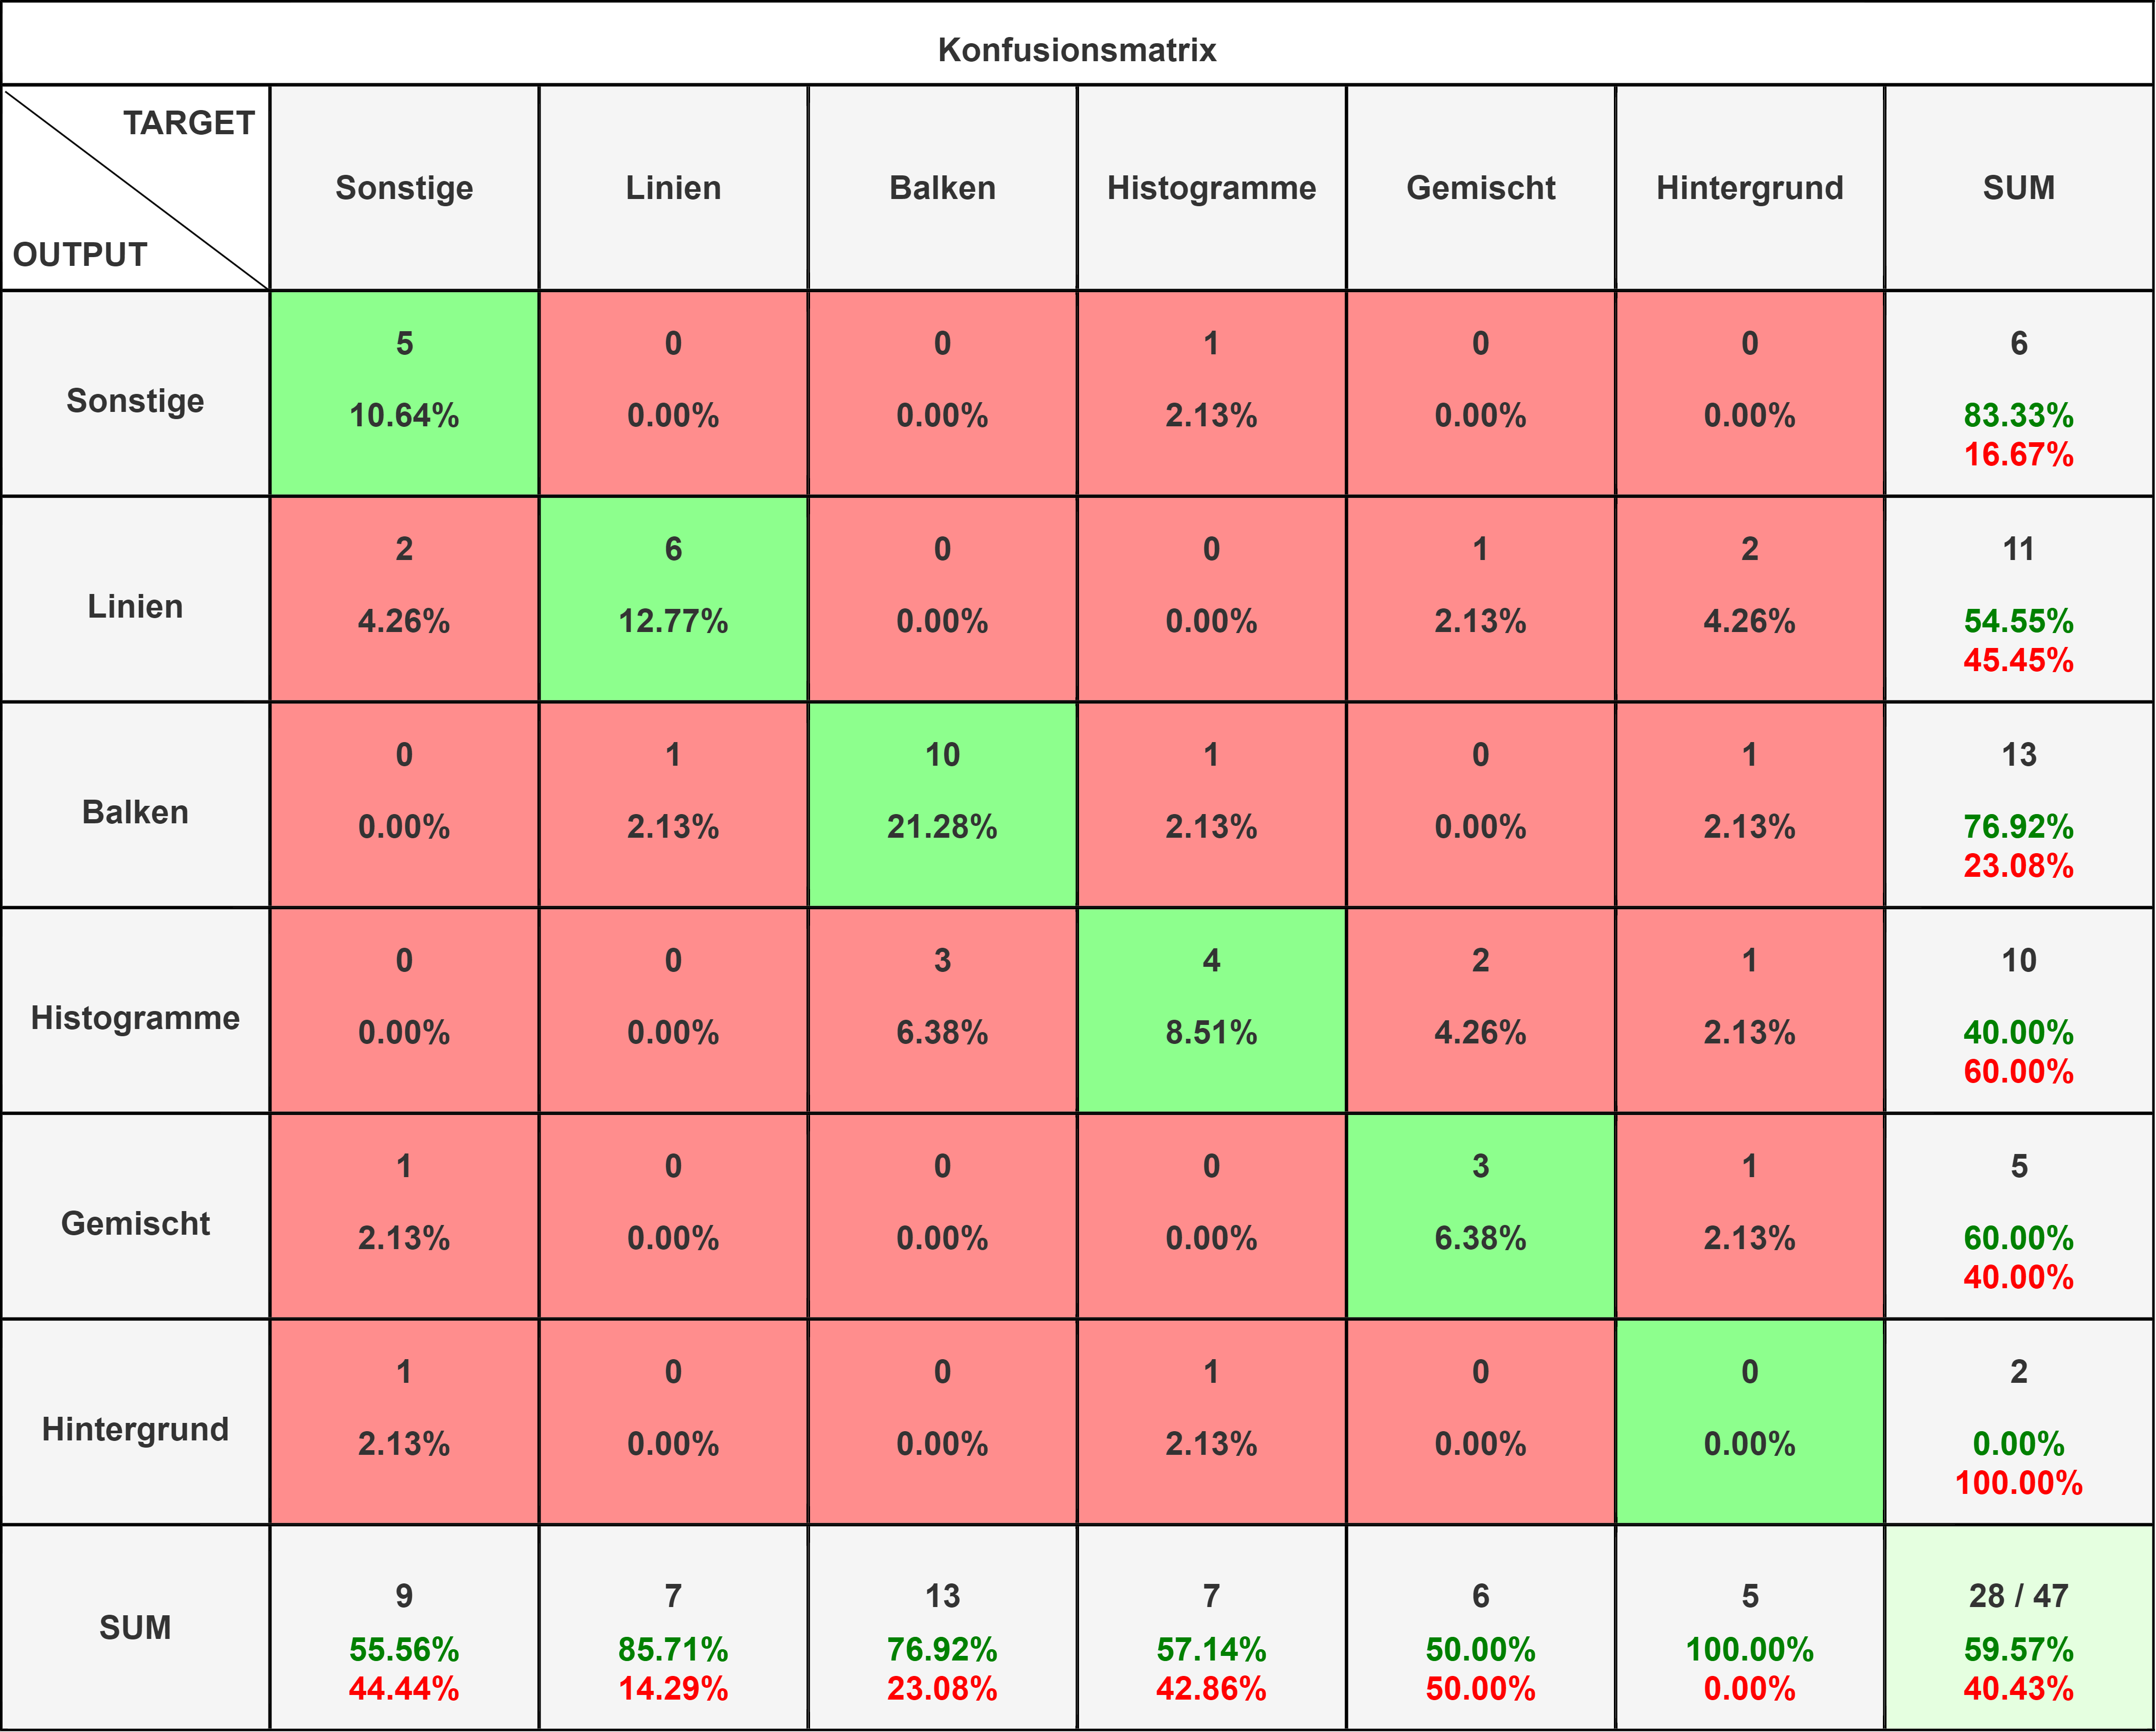
\includegraphics[width=1\textwidth]{Experimente/img/detect/1_val@0.404_200_histo/konfusionsmatrix.png}
    \caption{\hbadness=10000 Konfusionsmatrix des Modells, trainiert auf 200 Trainingsbildern mit Histogramme}
    \label{fig:extraction_output}
\end{figure}

\begin{table}[H]
    \centering
    \begin{tabular}{|l|c|c|c|}
        \hline
        \rowcolor[HTML]{EFEFEF}
                      & Precision        & Recall           & F1-Score         \\ \hline
        Sonstige      & 83.33\%          & 55.56\%          & 66.67\%          \\ \hline
        Linien        & 54.55\%          & 85.71\%          & 66.67\%          \\ \hline
        Balken        & 76.92\%          & 76.92\%          & 76.92\%          \\ \hline
        Histogramme   & 40.00\%          & 57.14\%          & 47.06\%          \\ \hline
        Gemischt      & 60.00\%          & 50.00\%          & 54.55\%          \\ \hline
        \textbf{Alle} & \textbf{62.96\%} & \textbf{65.07\%} & \textbf{62.37\%} \\ \hline
    \end{tabular}
    \caption{Evaluationswerte des Modells, trainiert auf 200 Trainingsbildern mit Histogramme}
\end{table}


\subsection*{200 Trainingsbilder (ohne Histogramme)}
Mit einem Konfidenzwert von 51.1\% wurden folgende Ergebnisse des trainierten Modells auf den Datensatz der reduzierten Klassenanzahl erzielt. Auffallend sind nicht nur, der limitierten Evaluationsdatensatzgröße verschuldet, leichte Abweichungen der Linien und gemischten Klassen, sondern auch deutliche Verbesserungen der nun zusammengesetzten Balkendiagramme.

\begin{figure}[H]
    \centering
    \captionsetup{width=1\linewidth}
    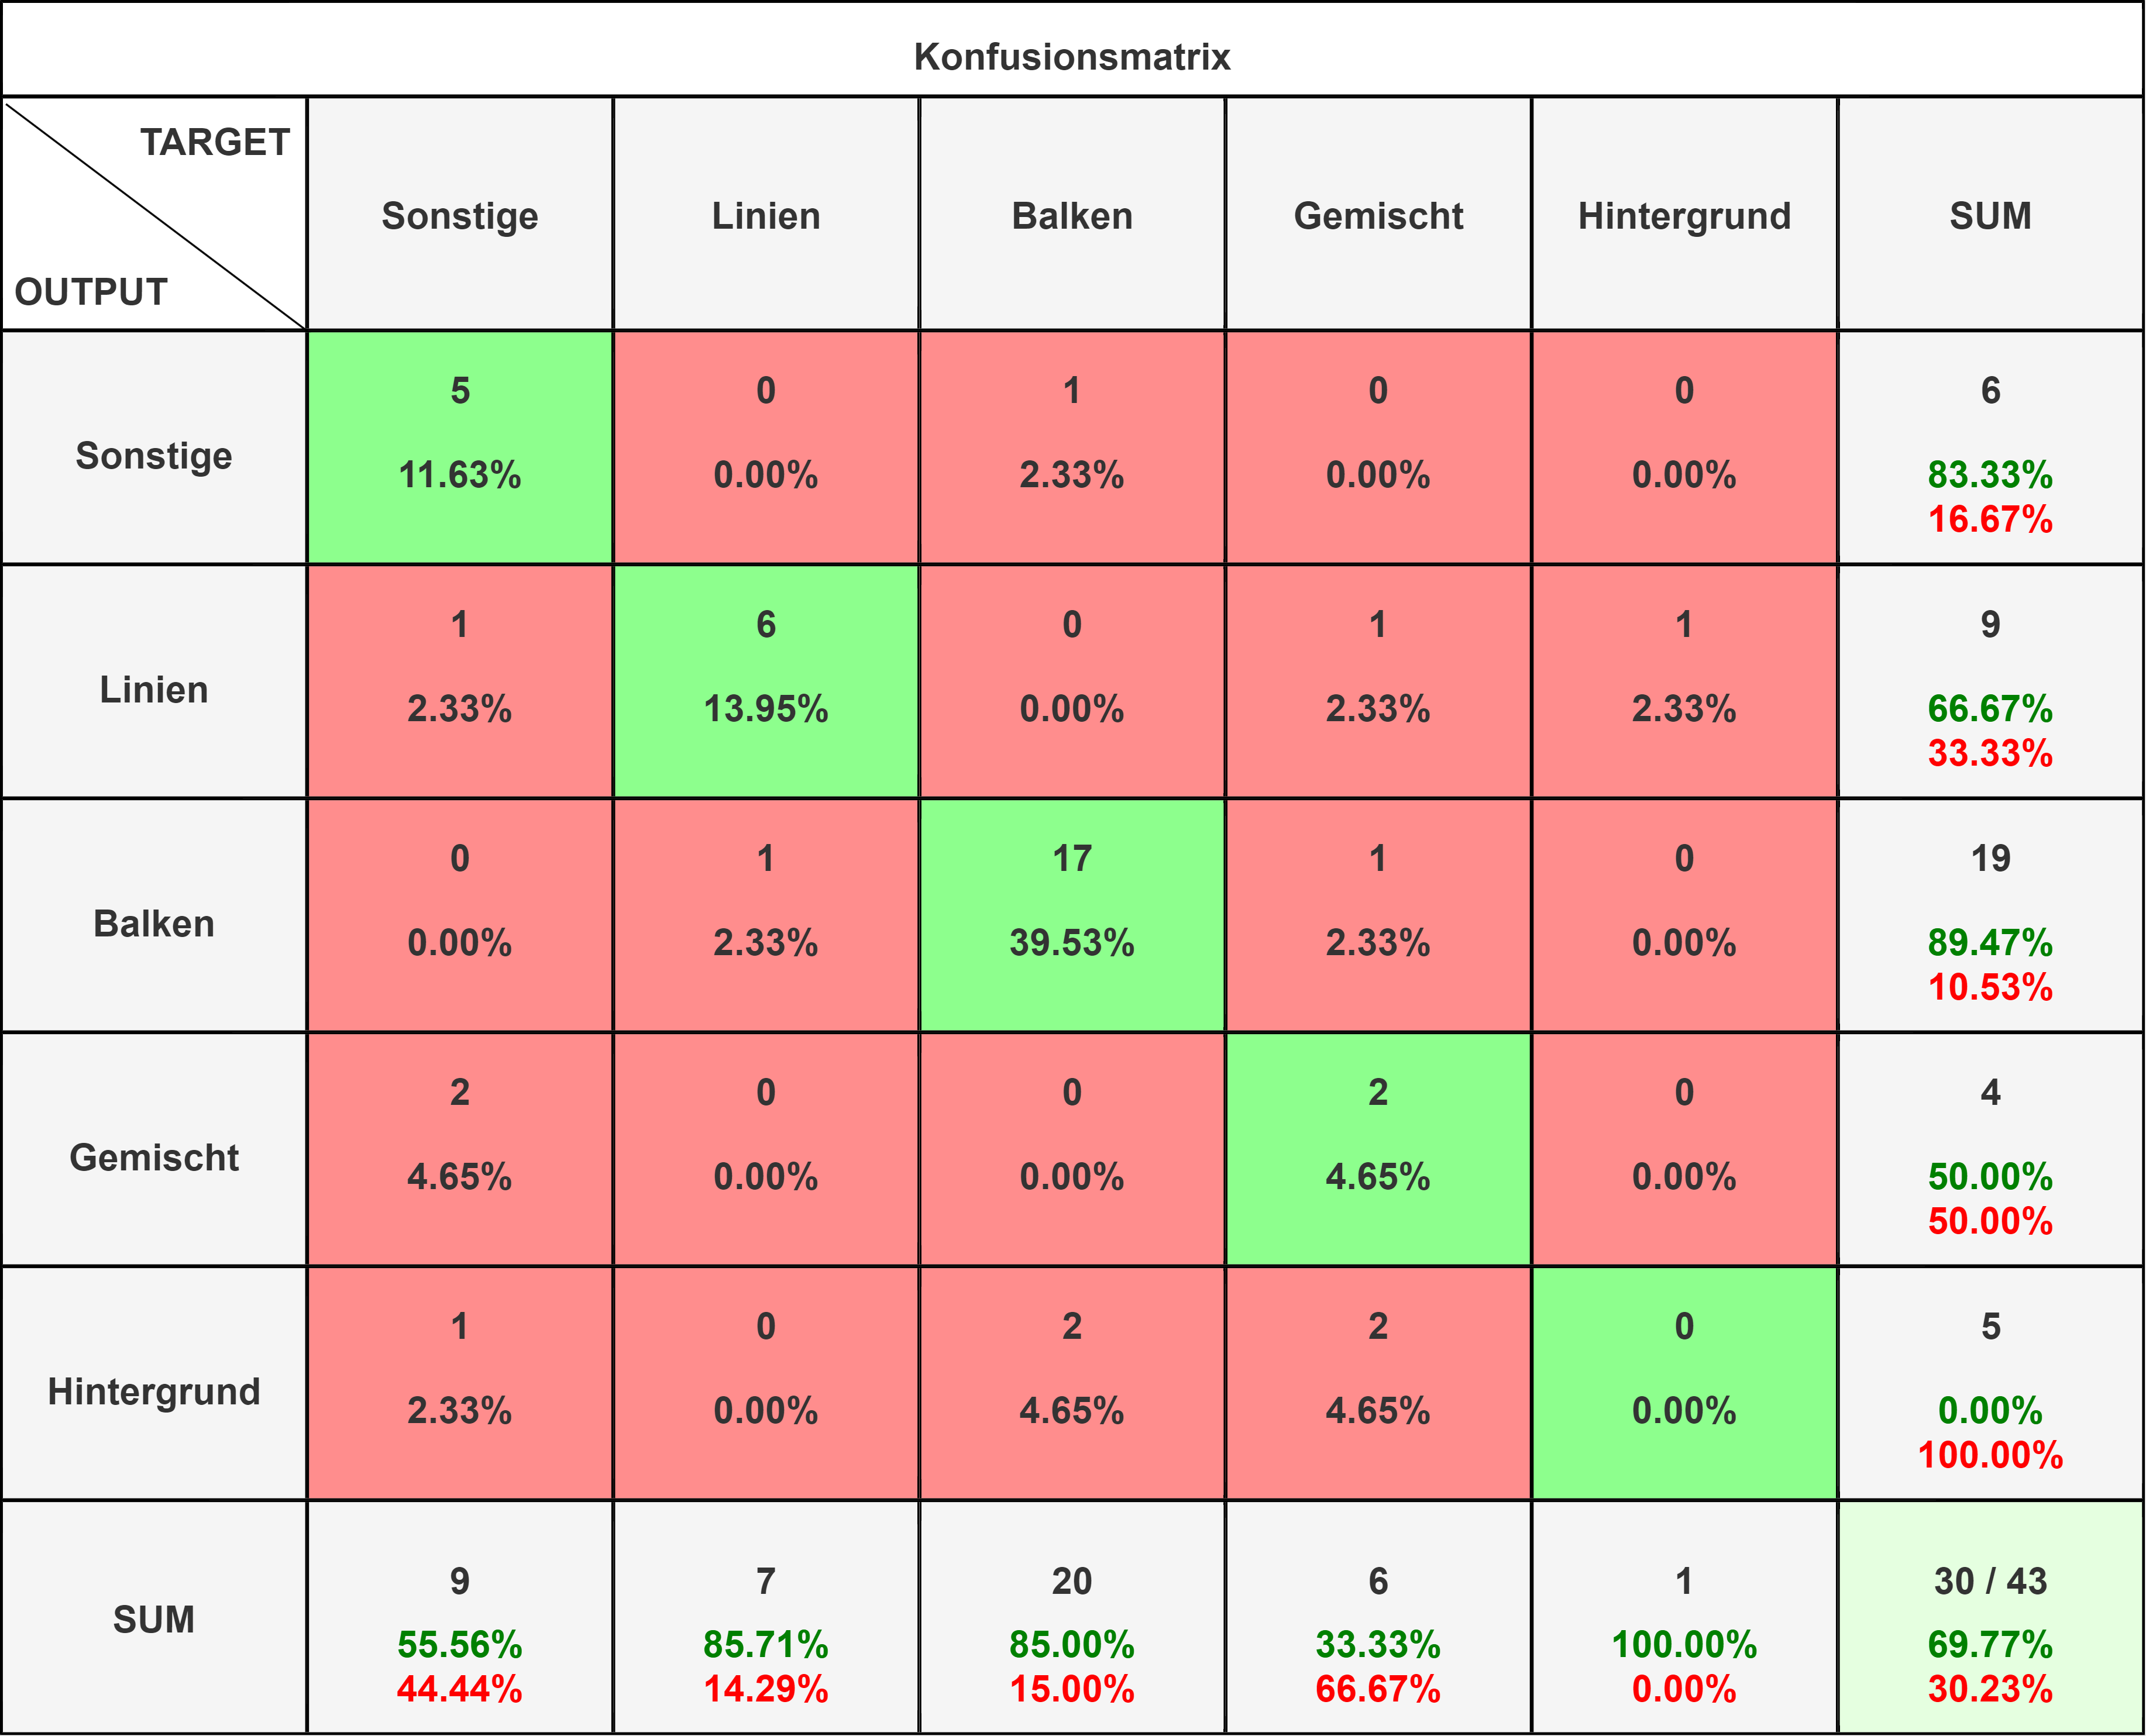
\includegraphics[width=1\textwidth]{Experimente/img/detect/2_val@0.511_200_nohisto/konfusionsmatrix.png}
    \caption{\hbadness=10000 Konfusionsmatrix des Modells, trainiert auf 200 Trainingsbildern ohne Histogramme}
    \label{fig:extraction_output}
\end{figure}

\begin{table}[H]
    \centering
    \begin{tabular}{|l|c|c|c|}
        \hline
        \rowcolor[HTML]{EFEFEF}
                      & Precision        & Recall           & F1-Score         \\ \hline
        Sonstige      & 83.33\%          & 55.56\%          & 66.67\%          \\ \hline
        Linien        & 66.67\%          & 85.71\%          & 75.00\%          \\ \hline
        Balken        & 89.47\%          & 85.00\%          & 87.18\%          \\ \hline
        Gemischt      & 50.00\%          & 33.33\%          & 40.00\%          \\ \hline
        \textbf{Alle} & \textbf{72.37\%} & \textbf{64.90\%} & \textbf{67.21\%} \\ \hline
    \end{tabular}
    \caption{Evaluationswerte des Modells, trainiert auf 200 Trainingsbildern ohne Histogramme}
\end{table}

\subsection*{321 Trainingsbilder}
Nach der Entscheidung, Histogramme und Balkendiagramme zu kombinieren, wurde mit dem finalen Datensatz von 321 annotierten Bildern schließlich das endgültige Modell vortrainiert. Da mit einem größeren Datensatz die Anzahl der Validationsbilder auch ansteigt, sind diese Evaluationen nun vertraulicher. Auffallend ist jedoch die deutlich schlechter ausfallende Recall-Metrik bei dem gewählten Confidence Threshold von 65.3\%. Das Hauptziel dieses Modells ist jedoch lediglich das Vortrainieren, weshalb die vorliegenden Ergebnisse weniger kritisch begutachtet werden können als das eigentliche feintrainierte Modell. Grundsätzlich ist jedoch herauszunehmen, dass eine Trainingsbildgröße von 321 ungenügend ist.

\begin{figure}[H]
    \centering
    \captionsetup{width=1\linewidth}
    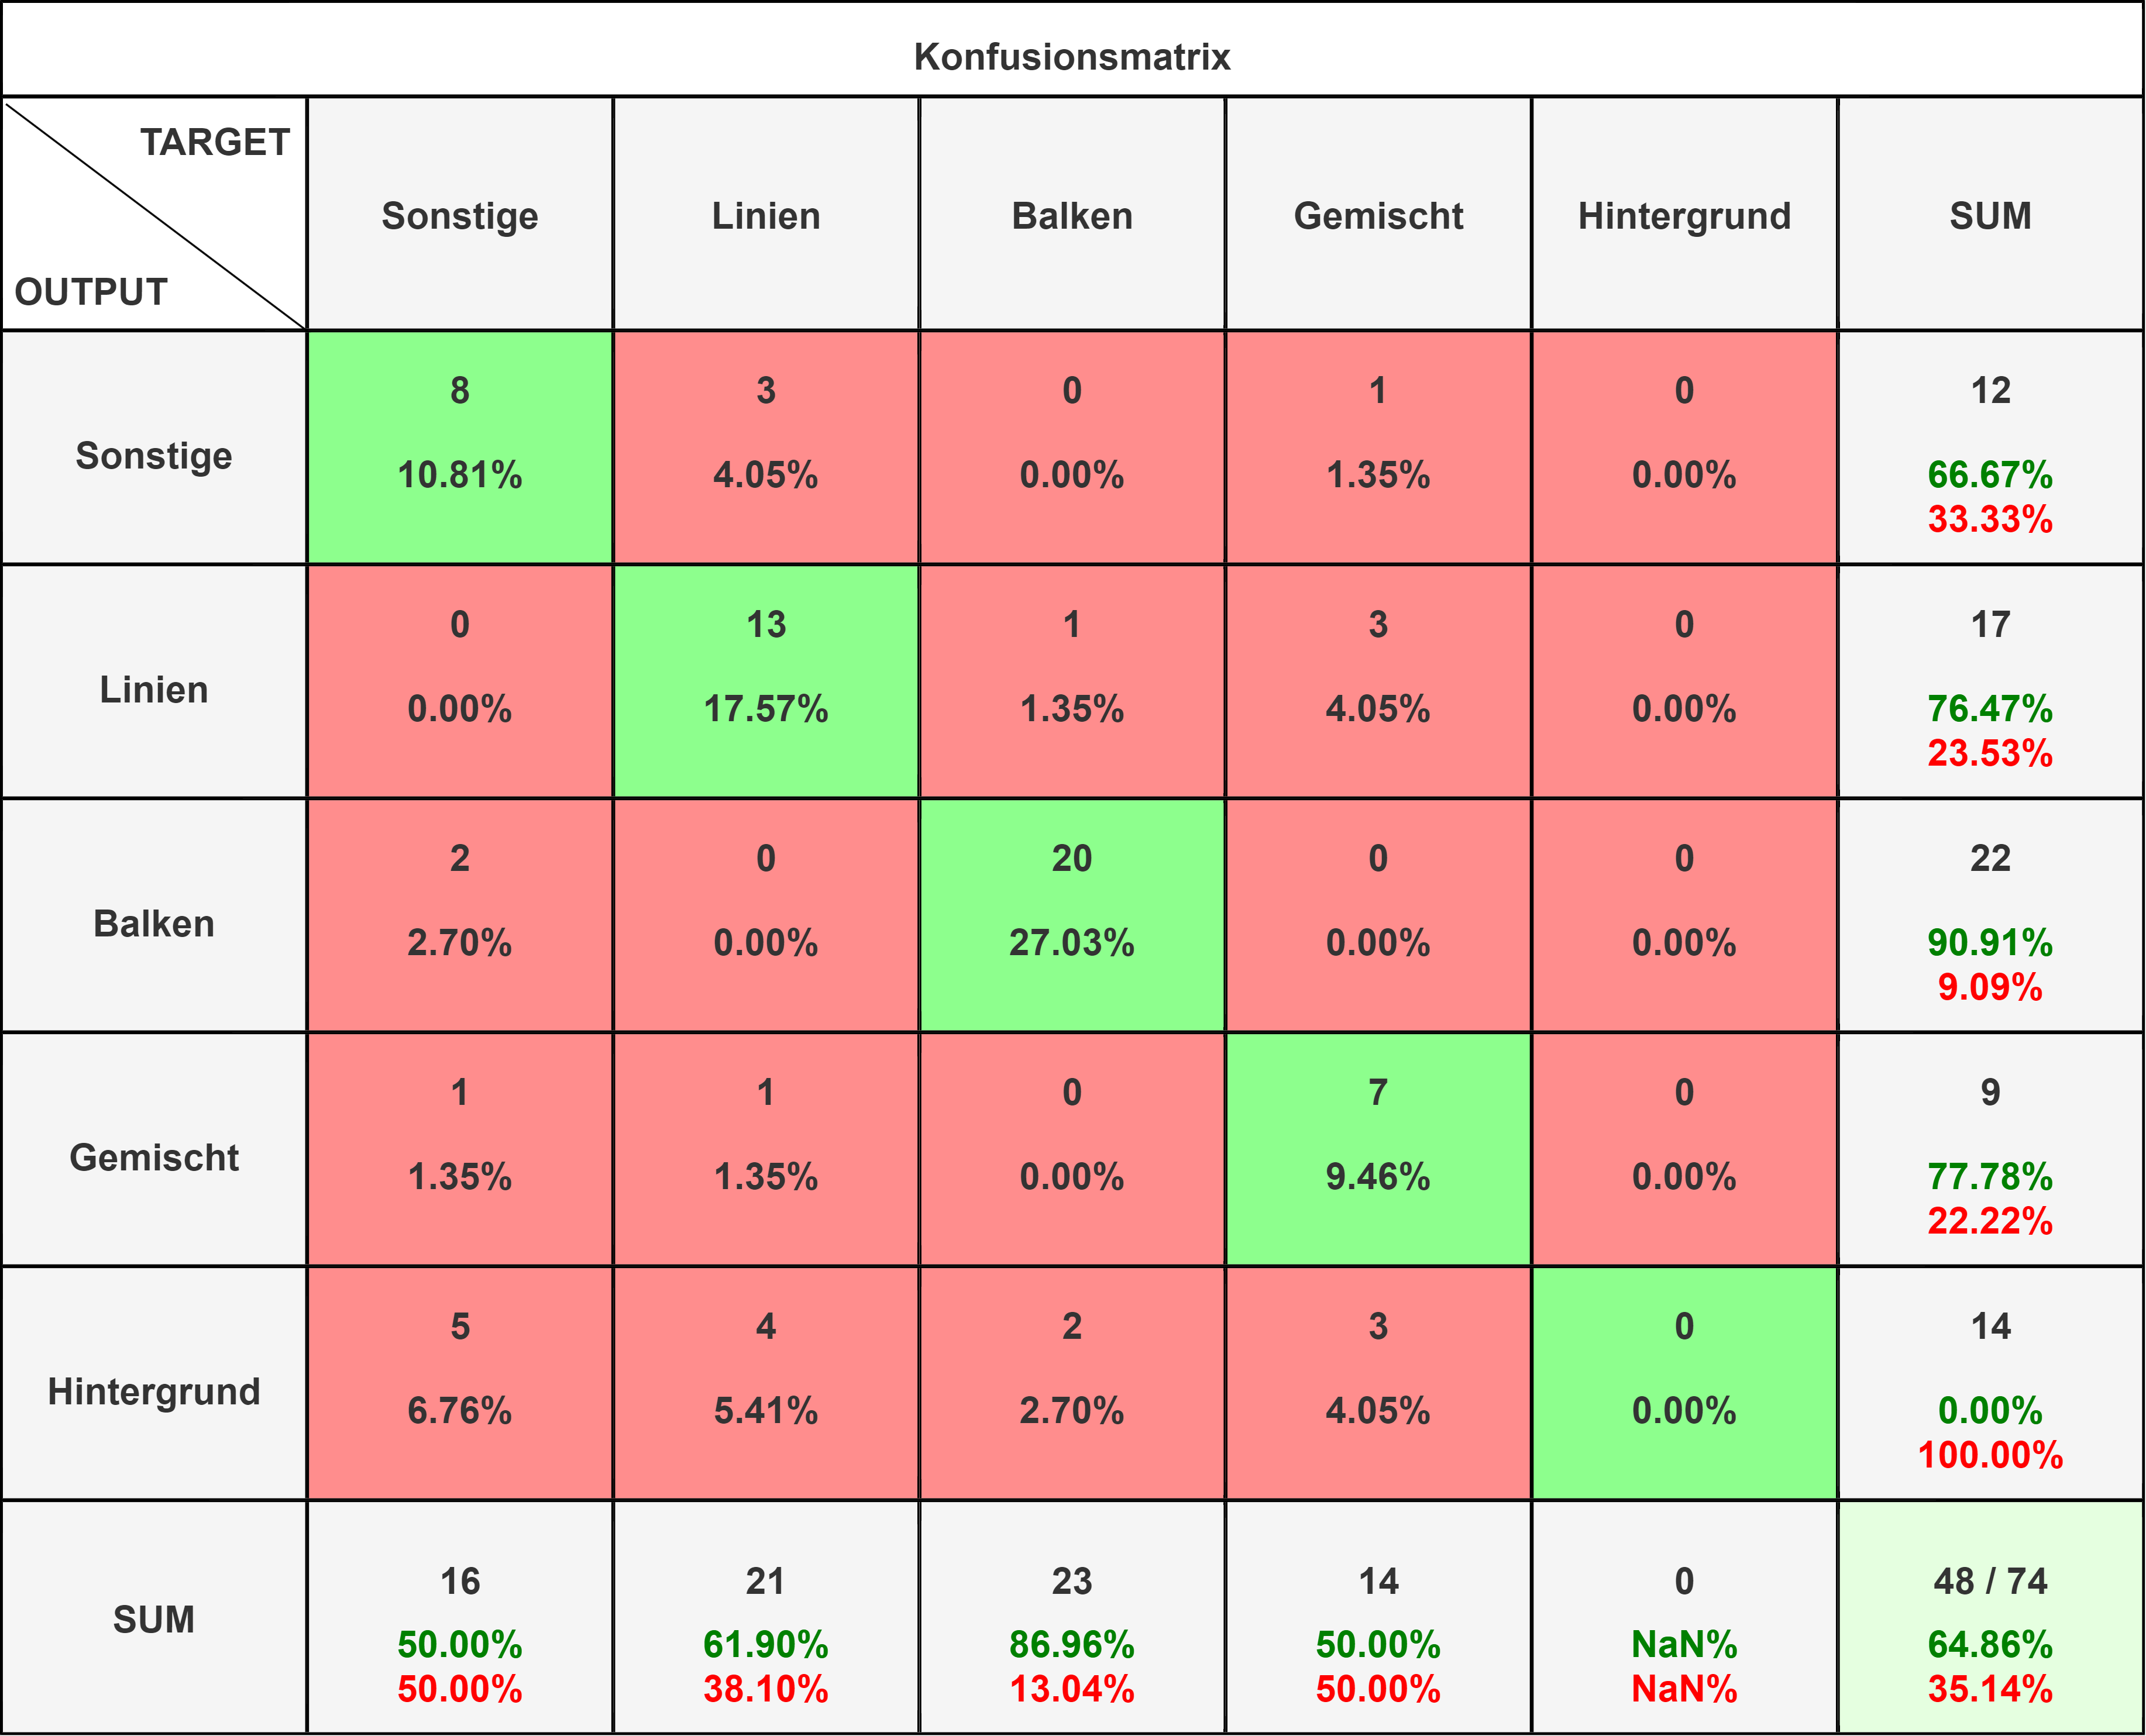
\includegraphics[width=1\textwidth]{Experimente/img/detect/3_val@0.653_nohisto/konfusionsmatrix.png}
    \caption{\hbadness=10000 Konfusionsmatrix des Modells, trainiert auf 321 Trainingsbildern}
    \label{fig:extraction_output}
\end{figure}

\begin{table}[H]
    \centering
    \begin{tabular}{|l|c|c|c|}
        \hline
        \rowcolor[HTML]{EFEFEF}
                      & Precision        & Recall           & F1-Score         \\ \hline
        Sonstige      & 66.67\%          & 50.00\%          & 57.14\%          \\ \hline
        Linien        & 76.47\%          & 61.90\%          & 68.42\%          \\ \hline
        Balken        & 90.91\%          & 86.96\%          & 88.89\%          \\ \hline
        Gemischt      & 77.78\%          & 50.00\%          & 60.87\%          \\ \hline
        \textbf{Alle} & \textbf{77.96\%} & \textbf{62.22\%} & \textbf{68.83\%} \\ \hline
    \end{tabular}
    \caption{Evaluationswerte des Modells, trainiert auf 321 Trainingsbildern}
\end{table}


\subsection{Feintraining auf historische Wirtschaftsscans}

Im Anschluss wurde das vortrainierte Modell verwendet, um das Feintrainieren auf dem erstellten Datensatz der historischen Wirtschaftsmagazine auszuführen.

\subsection*{2444 Trainingsbilder}
Die Metriken wurden mit einem Konfidenzwert von 89.1\% evaluiert. Aus der Konfusionsmatrix lassen sich die Klassenverteilungen ablesen, wobei die Liniendiagrammsklasse hier eindeutig überwiegt. Dies spiegelt sich auch in der Tabelle wider, bei der nur bei der Klasse der Linien sich ein ausgewogener Precision- und Recall-Wert auslesen lässt. Die geringe Existenz der Nicht-Linien-Diagramme in den Wirtschaftsscans lässt so nur die glaubwürdige Evaluation der Liniendiagramme selbst zu, welche mit einer Precision von 95.83\% und Recall von 94.52\% auch gute Ergebnisse liefert, weshalb im weiteren Verlauf der Arbeit sich nur auf die Auswertung dieser fokusiert wurde.

\begin{figure}[H]
    \centering
    \captionsetup{width=1\linewidth}
    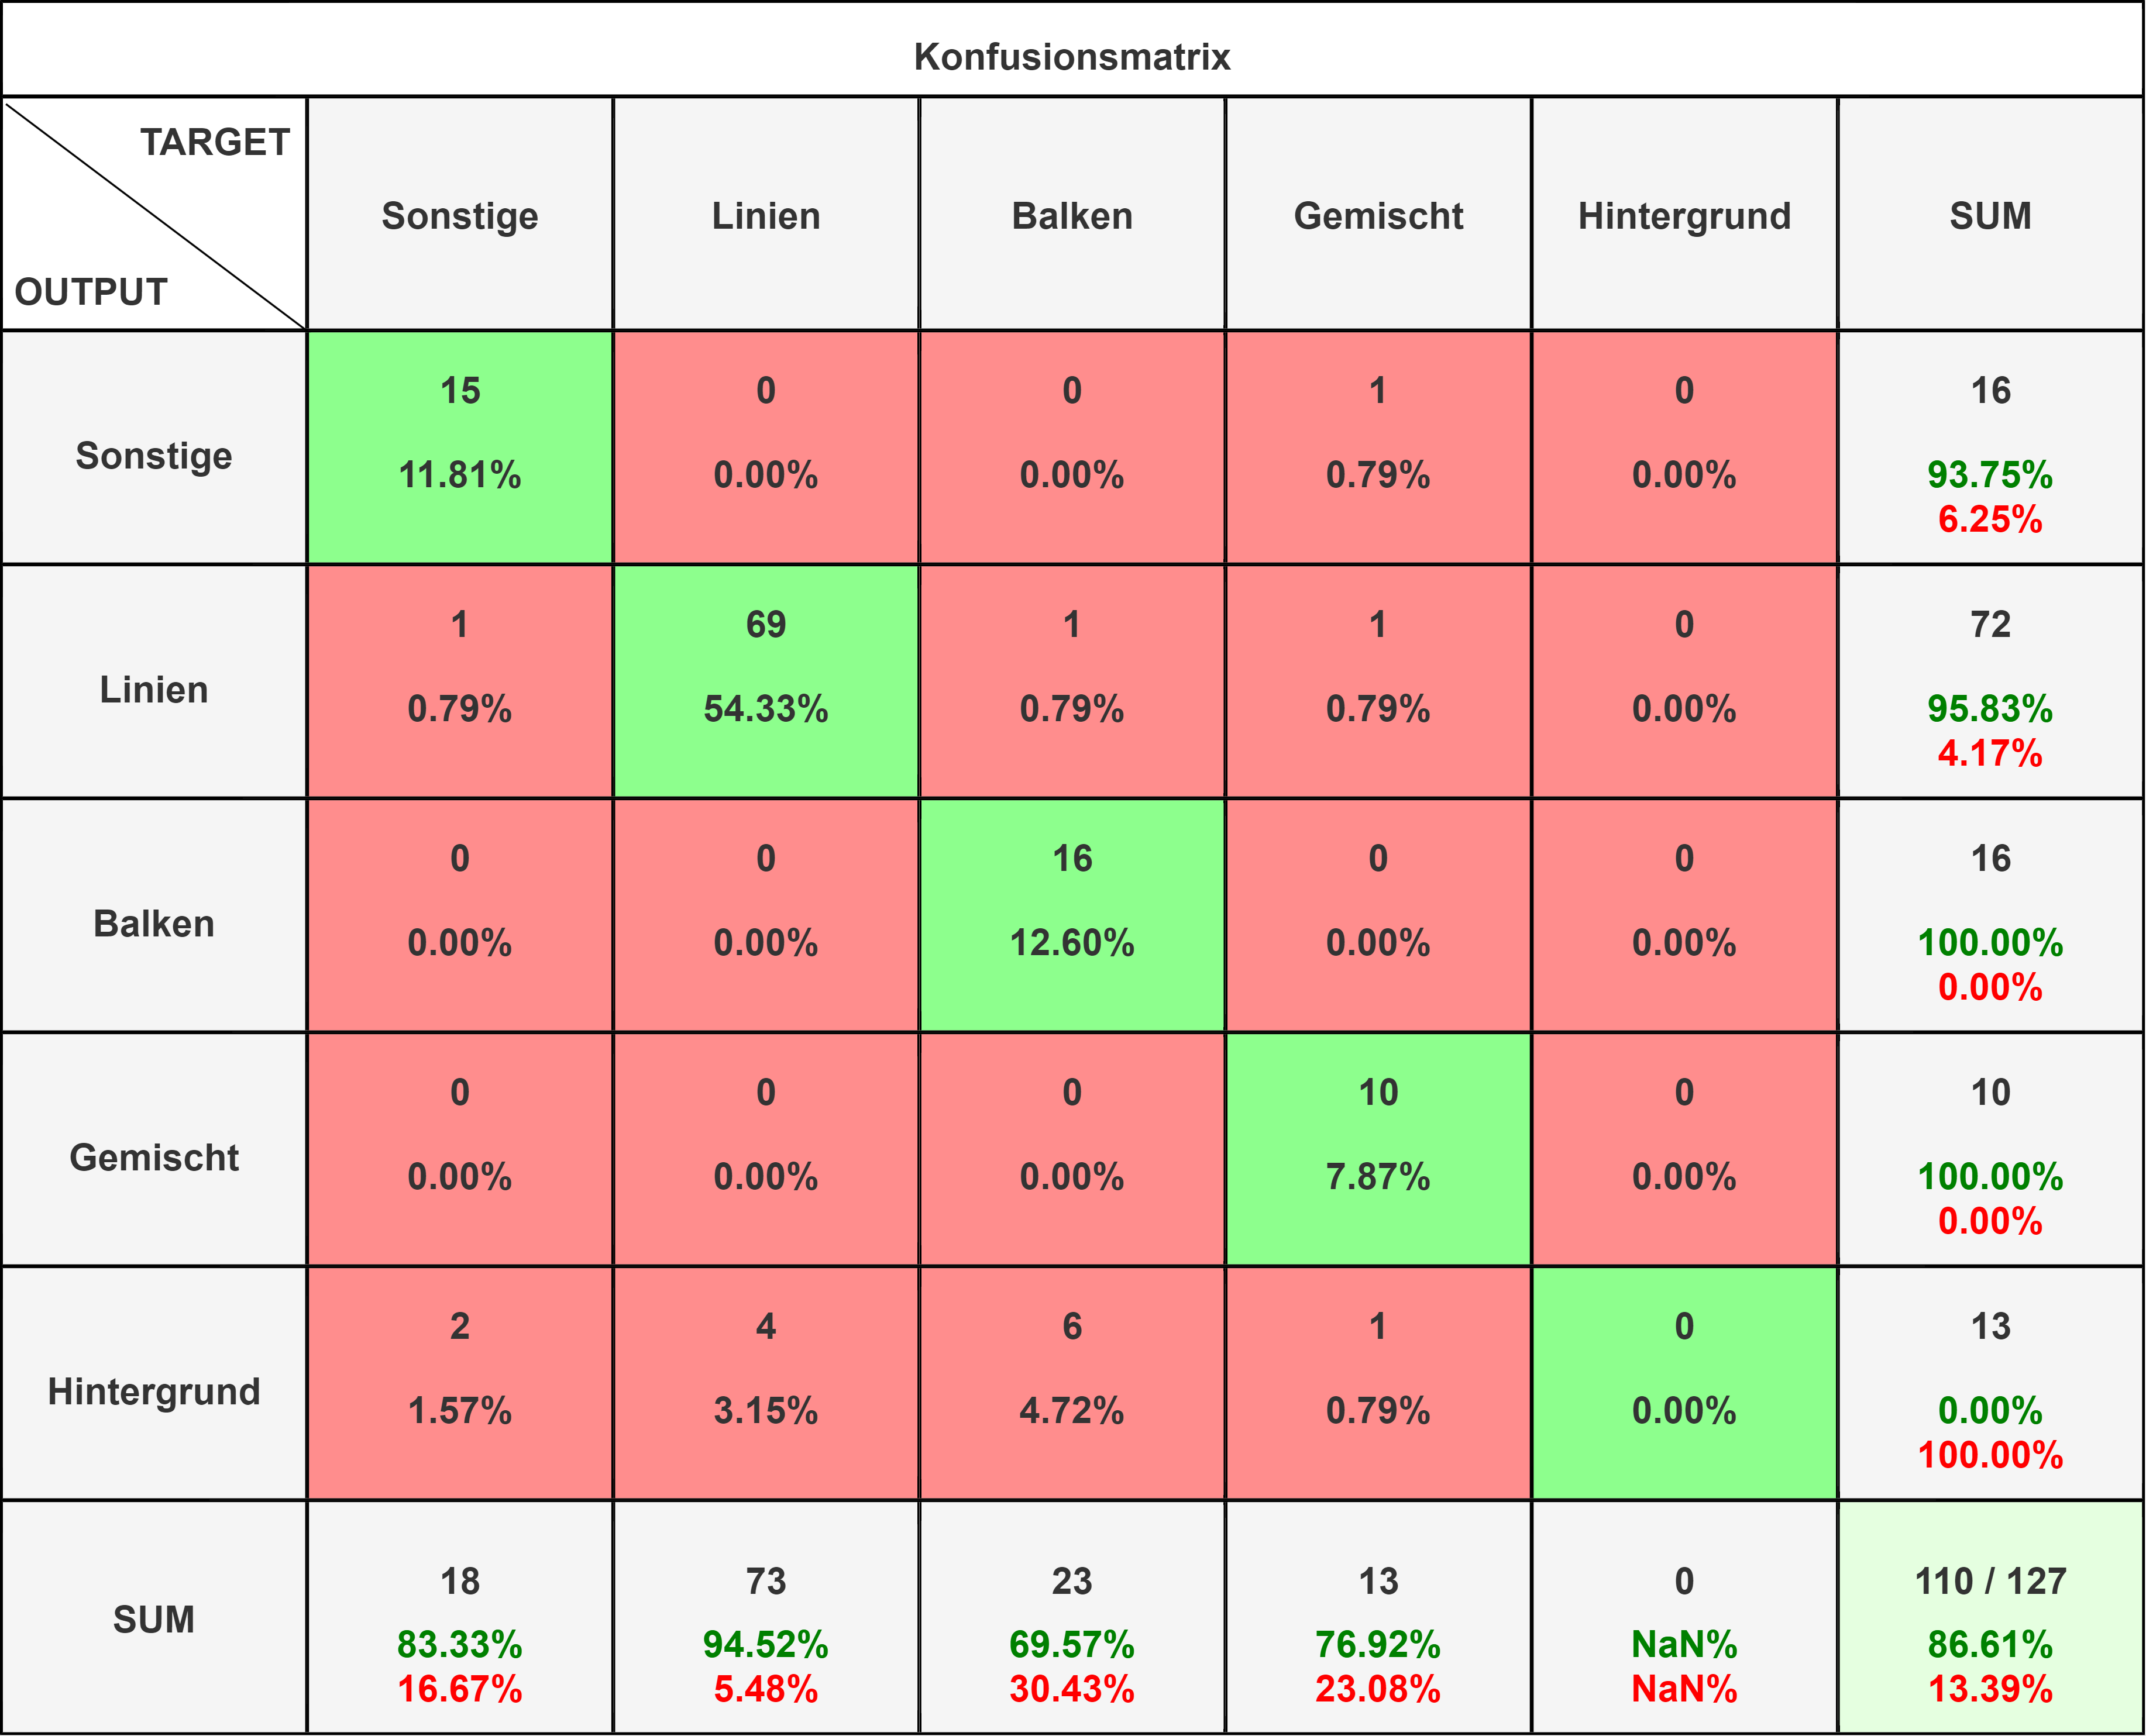
\includegraphics[width=1\textwidth]{Experimente/img/detect/val@0.891 20240612-093743_double/konfusionsmatrix.png}
    \caption{\hbadness=10000 Konfusionsmatrix des feintrainierten Modells}
    \label{fig:extraction_output}
\end{figure}

\begin{table}[H]
    \centering
    \begin{tabular}{|l|c|c|c|}
        \hline
        \rowcolor[HTML]{EFEFEF}
                      & Precision        & Recall           & F1-Score         \\ \hline
        Sonstige      & 93.75\%          & 83.33\%          & 88.24\%          \\ \hline
        Linien        & 95.83\%          & 94.52\%          & 95.17\%          \\ \hline
        Balken        & 100.0\%          & 69.57\%          & 82.05\%          \\ \hline
        Gemischt      & 100.0\%          & 76.92\%          & 86.96\%          \\ \hline
        \textbf{Alle} & \textbf{97.40\%} & \textbf{81.09\%} & \textbf{88.11\%} \\ \hline
    \end{tabular}
    \caption{Evaluationswerte des feintrainierten Modells}
\end{table}


\section{Liniendiagrammsklassifizierung}
\label{ch:classify_eval}

Für die Liniendiagrammsklassifizierung wurden zwei Modelle jeweils auf die erstellten Datensätze aus \ref{ch:linebank} trainiert. Die Konfusionsmatrix in Abbildung \ref{fig:val_v1_matrix} macht die Schwierigkeit des Modells deutlich, überlappende und nicht überlappende Liniendiagramme zu differenzieren. Im Gegensatz zu \ref{fig:val_v2_matrix} werden hier 7 der insgesamt 19 nicht überlappenden Aufkommen falsch als überlappende Diagramme klassifiziert.

\begin{figure}[H]
    \centering
    \captionsetup{width=.75\linewidth}
    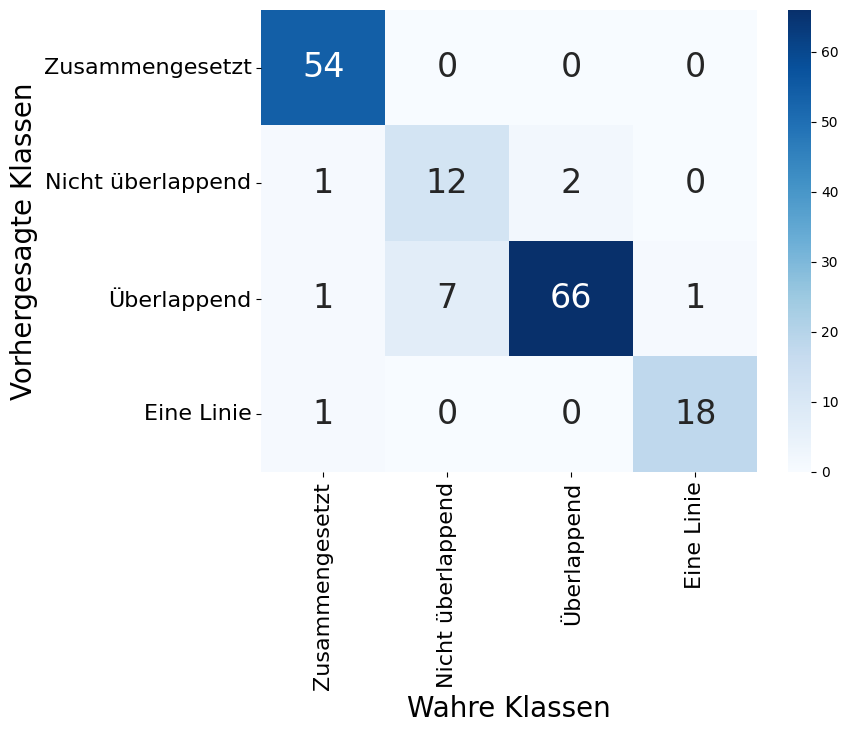
\includegraphics[width=.75\textwidth]{Experimente/img/classify/val_v1/matrix.png}
    \caption{\hbadness=10000 Konfusionsmatrix des Datensatzes mit überlappenden und nicht überlappenden Liniendiagramme}
    \label{fig:val_v1_matrix}
\end{figure}

Die besseren Ergebnisse der Unterscheidung zwischen einer und mehreren Wertelinien spiegeln sich aber auch in der Accuracy wider: Statt 92.0\% des ersten Modells erzielte dieses eine Klassifikationsgenauigkeit von 98.1\%.

\begin{figure}[H]
    \centering
    \captionsetup{width=.75\linewidth}
    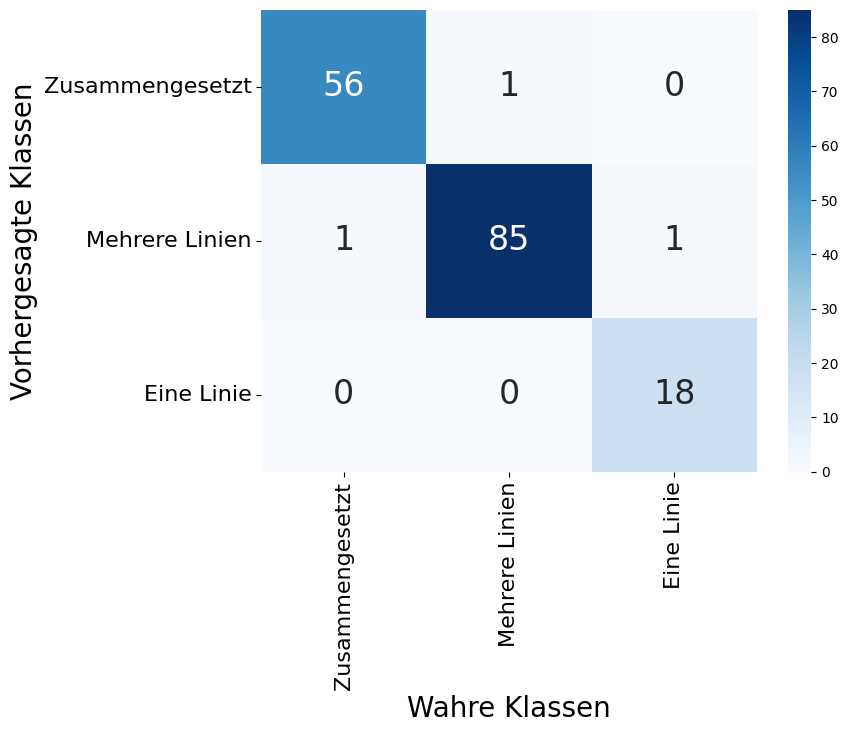
\includegraphics[width=.75\textwidth]{Experimente/img/classify/val_v2/matrix.png}
    \caption{\hbadness=10000 Konfusionsmatrix des reduzierten Datensatzes}
    \label{fig:val_v2_matrix}
\end{figure}

\section{Segmentation}

Für die Wertelinienerkennung werden in diesem Unterkapitel beide Segmentierungsansätze evaluiert. Da die Instanzsegmentation neben der Maske ebenfalls getrennte Linien produziert, können schwer genaue Vergleiche zwischen den zwei gezogen werden. Nichtsdestotrotz lassen sich die produzierten Maskenvorhersagen zumindest trotzdem durch Precision und Recall gegenüberstellen.


\subsection{Instanzsegmentation durch Ultralytics YOLO}

Das feintrainierte Modell wurde dem F1-Score maximierend mit einem Confidence Threshold von 51,11\% evaluiert. Aufgrund der Instanzsegmentation stellt Ultralytics hierfür nicht nur die Maskenevaluation, sondern auch die Bewertung des Begrenzungsrechtecks (bounding box) zur Verfügung. Der starke Unterschied zwischen Precision und Recall, selbst bei einem Schwellenwert von knapp 50\%, fällt hier auf. Oftmals kommt es dazu, dass ganze Linien nicht erkannt werden, was zu diesem reduzierten Recall-Wert führt. Das Problem der korrekten Linienanzahlerkennung wird im Folgenden weiter evaluiert.

\begin{table}[H]
    \centering
    \begin{tabular}{|l|c|c|c|}
        \hline
        \rowcolor[HTML]{EFEFEF}
              & Precision & Recall & F1-Score \\ \hline
        Box   & 95.6\%    & 78.8\% & 86.4\%   \\ \hline
        Maske & 93.3\%    & 76.4\% & 84.0\%   \\ \hline
    \end{tabular}
    \caption{Metrikwerte des feintrainierten Ultralytics YOLO Modells}
\end{table}

Um die korrekte Linienkontinuität der es auszeichnend machenden Instanzsegmentation zu untersuchen wurden 63 zufällig ausgewählte Liniendiagramme in drei Kategorien differenziert: Einfache Diagramme mit maximal wenig und deutlichen Linienüberschneidungen, Mittelschwere mit mehr Überlschneidungen oder Überlappungen der Wertelinien, welche jedoch aufgrund ihrer visuellen Darstellung klar unterscheiden werden könnnen und schwere Diagramme für die restlichen Diagramme mit vielen sich überschneidenen Linien, die teils auch bei manueller menschlicher Bewertung zu Schwierigkeiten führen.

\begin{figure}[H] % or any other figure positioning (H, h, t, b)
    \centering
    \begin{minipage}{0.315\textwidth} % First figure
        \centering
        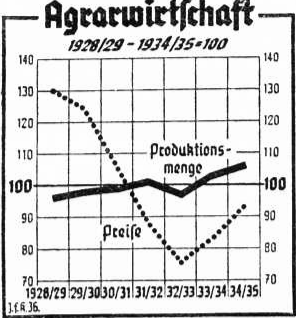
\includegraphics[width=\linewidth]{Experimente/img/easy.png}
        \caption{\hbadness=10000 Einfaches Liniendiagramm}
        \label{fig:easy}
    \end{minipage}\hfill % Add space between figures 
    \begin{minipage}{0.315\textwidth} % Second figure 
        \centering
        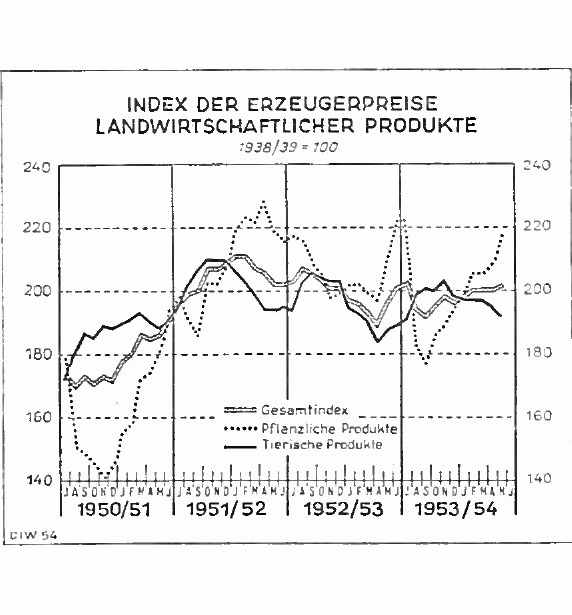
\includegraphics[width=\linewidth]{Experimente/img/medium.png}
        \caption{\hbadness=10000 Mittelschweres Liniendiagramm}
        \label{fig:medium}
    \end{minipage}\hfill % Add space between figures
    \begin{minipage}{0.315\textwidth} % Second figure
        \centering
        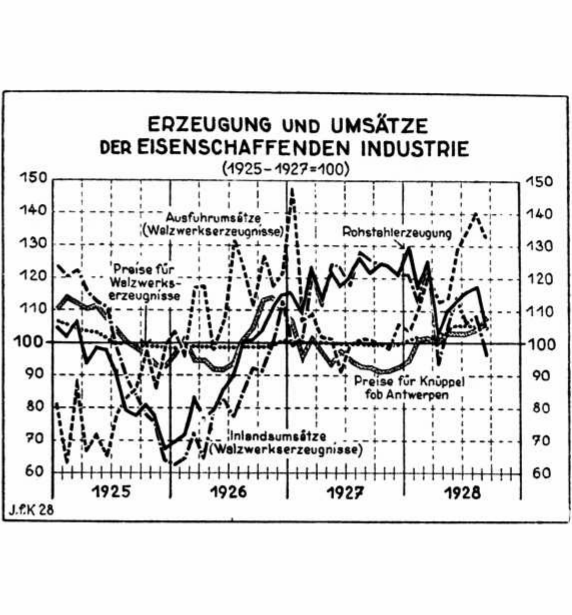
\includegraphics[width=\linewidth]{Experimente/img/hard.png}
        \caption{\hbadness=10000 Schweres Liniendiagramm}
        \label{fig:hard}
    \end{minipage}
\end{figure}

Ebenfalls wurde bei der Evaluation die korrekt erkannte Linienanzahl bewertet, da die Instanzsegmentation im Vergleich zu der folgenden semantischen Segmentation der Architektur verschuldet oft ganze Linien auslässt wie oben bereits durch den niedrigeren Recall Wert widerspiegelend.
Die unrealisierbare korrekte Erkennung der schweren Liniendiagrammen ist hier kaum überraschend, manche dieser wären auch einen Menschen unöglich. Interessanter sind allerdings die Klassen der einfachen und mittelschweren Diagramme. Die korrekte Linienfortführung führt hier zu andwendbareren Ergebnissen, wobei auf die korrekte Linienanzahlerkennung des Modells sich wenig verlassen werden kann.

\begin{table}[H]
    \centering
    \begin{minipage}{0.475\textwidth}
        \centering
        \begin{tabular}{|l|c|c|c|}
            \hline
            \rowcolor[HTML]{EFEFEF}
                    & Einfache & Mittlere & Schwere \\ \hline
            Korrekt & 21       & 18       & 0       \\ \hline
            Falsch  & 1        & 10       & 13      \\ \hline
        \end{tabular}
        \caption{Korrekte Linienfortführung \phantom{Platzhalter}}
    \end{minipage}%
    \hfill
    \begin{minipage}{0.475\textwidth}
        \centering
        \begin{tabular}{|l|c|c|c|}
            \hline
            \rowcolor[HTML]{EFEFEF}
                    & Einfache & Mittlere & Schwere \\ \hline
            Korrekt & 17       & 10       & 0       \\ \hline
            Falsch  & 5        & 18       & 13      \\ \hline
        \end{tabular}
        \caption{Davon Linienanzahl richtig erkannt}
    \end{minipage}
\end{table}

\subsection{Semantische Segmentation durch das U-Net}
\label{ch:eval_unet}

Mit den genannten Parametern aus \ref{ch:unet} wurden insgesamt fünf verschiedene Modelle trainiert: Eines wurde auf den in \ref{ch:lines} beschriebenen Binärmaskendatensatz der Wertelinien von synthetischen Liniendiagrammen vortrainiert. Die restlichen vier Modelle wurden auf den Werteliniendatensatz der historischen Liniendiagramme so trainiert, um jeweils den Vergleich zwischen dem Fein- und nicht Feintrainieren und der selbst eingeführten Beschreibung des \emph{32x Batch-Padding} darzustellen. Was dieses Batch-Padding beschreibt, ist lediglich die 32-fache Duplikation aller einzelnen Trainingsdatenbilder. Da jeder einzelne Bilderbatch während des Trainingsprozesses zufällig neu augmentiert wird und so durch das Batch-Padding die limitierten Trainingsdaten möglicherweise künstlich vergrößert werden könnten, wurde dies untersucht.
\\
Alle im Folgenden dargestellten Ergebnisse wurden auf demselben Validierungsdatensatz der historischen Diagrammswertelinien evaluiert. Um die Effizienz des erstellten Datensatzgenerators anschaulich zu machen, wurde das auf den synthetischen Bildern vortrainierte Modell ebenfalls auf diesem Validierungsdatensatz gemessen. Allerdings wurden hier keine herausragenden Evaluationswerte erwartet, da synthetische Datensätze in der Regel nicht die Qualität von realen Daten erreichen können.

\begin{table}[H]
    \centering
    \begin{minipage}{0.475\textwidth}
        \centering
        \begin{tabular}{|l|c|c|c|}
            \hline
            \rowcolor[HTML]{EFEFEF}
                  & Precision & Recall  & F1-Score \\ \hline
            Maske & 75.55\%   & 66.19\% & 70.56\%  \\ \hline
        \end{tabular}
        \caption{Training auf synthetischem Datensatz}
    \end{minipage}%
\end{table}

Die Tauglichkeit dieser künstlichen Herangehensweise zum lediglichen Vortrainieren spiegelt sich jedoch in den unteren Tabellen wider. Besonders der Precision-Wert zwischen vor- und nicht vortrainierten Modellen zeigt Verbesserungen, hier in beiden Fällen von fast 1.5\%. Recall scheint davon nicht ganz betroffen zu sein; die Verbesserungen bei dem einen und Verschlechterungen bei dem anderen können allerdings den Zufälligkeitsfaktoren des Trainings verschuldet sein. Die gleichen Auffälligkeiten können im Fall des Batch-Padding gefunden werden.

\begin{table}[H]
    \centering
    \begin{minipage}{0.475\textwidth}
        \centering
        \begin{tabular}{|l|c|c|c|}
            \hline
            \rowcolor[HTML]{EFEFEF}
                  & Precision & Recall  & F1-Score \\ \hline
            Maske & 91.52\%   & 89.36\% & 90.43\%  \\ \hline
        \end{tabular}
        \caption{Training auf vortrainiertem Modell mit 32x Batch-Padding}
    \end{minipage}%
    \hfill
    \begin{minipage}{0.475\textwidth}
        \centering
        \begin{tabular}{|l|c|c|c|}
            \hline
            \rowcolor[HTML]{EFEFEF}
                  & Precision & Recall  & F1-Score \\ \hline
            Maske & 90.41\%   & 89.57\% & 89.99\%  \\ \hline
        \end{tabular}
        \caption{Training auf vortrainiertem Modell ohne 32x Batch-Padding}
    \end{minipage}

    \vspace{1.5em} % Adjust the spacing between the rows if needed

    \begin{minipage}{0.475\textwidth}
        \centering
        \begin{tabular}{|l|c|c|c|}
            \hline
            \rowcolor[HTML]{EFEFEF}
                  & Precision & Recall  & F1-Score \\ \hline
            Maske & 89.07\%   & 89.64\% & 89.35\%  \\ \hline
        \end{tabular}
        \caption{Training auf nicht vortrainiertem Modell mit 32x Batch-Padding}
    \end{minipage}%
    \hfill
    \begin{minipage}{0.475\textwidth}
        \centering
        \begin{tabular}{|l|c|c|c|}
            \hline
            \rowcolor[HTML]{EFEFEF}
                  & Precision & Recall  & F1-Score \\ \hline
            Maske & 88.05\%   & 88.88\% & 88.46\%  \\ \hline
        \end{tabular}
        \caption{Training auf nicht vortrainiertem Modell ohne 32x Batch-Padding}
    \end{minipage}
\end{table}

\section{Diagrammauswertung}

Da sich die Diagrammauswertung aus der Werteliniensegmentation und Achsenerkennung durch OCR zusammensetzt, wurde nach obiger Evaluation des U-Nets ebenfalls die Effizienz des anderen Algorithmusteils beurteilt. Abgerundet wird das Kapitel der Experimente mit der Analyse des Diagrammauswertungsalgorithmus im Ganzen. Als Evaluationsdatensatz wurde für dieses gesamte Kapitel die durch \ref{ch:classify} implementierte und in \ref{ch:classify_eval} evaluierte Liniendiagrammsklassen der einer und mehreren Wertelinien verwendet. Wurden Instanzen dieser falsch klassifiziert, so wurden diese bei den folgenden Auswertungen ignoriert.

\subsection{Achsenerkennung durch OCR}
\label{ch:eval_ocr}

Die Funktionsweise der Achsenerkennung durch optische Schriftzeichenerkennung ist stark von der OCR selbst abhängig. Die Qualität der Erkennungen variiert stark durch die jeweilig verwendete OCR-Bibliothek, weswegen im Folgenden evaluierte Fehler in zwei, möglicherweise überlappende, Kategorien eingeteilt wurden. Diese bestehen aus den Fehlern des Algorithmus selbst, welche auch bei state-of-the-art Schriftzeichenerkennungsmethoden aufkommen würden. Da der Algorithmus das Auffinden der X-Achse im unteren Bildrand annimmt, kommen eventuelle Fehler dieser Kategorie durch Diagramme mit anderen X-Achsen-Positionen auf. Die andere Fehlergruppe ist der optischen Schriftzeichenerkennung selbst verschuldet, welche in Theorie durch eine bessere OCR-Bibliothek negiert werden kann.
\\
Es wurden 53 zufällige Diagramme manuell evaluiert, bei denen insgesamt 26 davon die korrekte Achsen- und Achsenbeschriftungserkennung erfüllten. Die Fehlerquellen der restlichen 27 Bilder werden in den unteren Tabellen dargestellt.

\begin{table}[H]
    \centering
    \begin{tabular}{|c|c|c|c|}
        \hline
        \rowcolor[HTML]{EFEFEF}
        Titel & Linke Y-Achse & Rechte Y-Achse & X-Achse \\ \hline
        3     & 0             & 1              & 7       \\ \hline
    \end{tabular}
    \caption{Von den 27 Fehlern wegen fehlerhaftem Achsenerkennungsalgorithmus}
    \label{tb:ocr1}
\end{table}

\begin{table}[H]
    \centering
    \begin{tabular}{|c|c|c|c|}
        \hline
        \rowcolor[HTML]{EFEFEF}
        Titel & Linke Y-Achse & Rechte Y-Achse & X-Achse \\ \hline
        6     & 6             & 4              & 10      \\ \hline
    \end{tabular}
    \caption{Von den 27 Fehlern wegen fehlerhafter optischer Schriftzeichenerkennung}
    \label{tb:ocr2}
\end{table}

\subsection{Numerische Tabellenformextraktion}

Letztendlich wurde der kombinierte und gesamte Tabellenformextraktionsalgorithmus evaluiert. Da der Algorithmus jedoch mit einigen Einschränkungen entworfen und seine einzigen Komponenten bereits oben in \ref{ch:eval_unet} und \ref{ch:eval_ocr} ausgewertet wurden, wurden einige Entscheidungen für die Algorithmusevaluation getroffen. Es soll die Effizienz des Algorithmus selbst bewertet werden, Fehler, die aufgrund von nicht ausgelegten Problemen entstehen, werden nicht in die Evaluation miteinbezogen. Folgende Annahmen wurden vorausgesetzt:
\\
Inkorrektheiten, verursacht durch die primitive Wertelinientrennung, bleiben unbeachtet, Fehler und Folgefehler der in \ref{ch:eval_ocr} beschriebenen optischen Schriftzeichenerkennung werden ignoriert und die Bewertung wird unabhängig des korrekten Linientitels der Legende durchgeführt. Außerdem werden alle Werte anhand der Mitte des jeweiligen X-Achsen-Labels abgelesen und nicht, wie korrekt, am eigentlichen respektiven Jahresende.
\\
Fehler werden durch den in \ref{ch:eval_ocr} genannten, fehlerhaften Achsenerkennungsalgorithmus gezählt, sowie bei falscher Y-Wert-Auswertung, die möglicherweise durch falsche Interpolation der Y-Achse bei Diagrammen mit beispielsweise logarithmischer Skala auftreten kann. Des Weiteren werden Fehler bei der falschen Werteliniensegmentation bestimmt, wie etwa beim Auftreten von Lücken oder irrtümlicher Erkennung in der Segmentierungsmaske.
\\
Insgesamt wurden 42 zufällig ausgewählte Liniendiagramme basierend auf den zuvor genannten Umständen manuell evaluiert.
\\
Die durchschnittliche Precision lag dabei bei 91.64\% und die des Recalls bei 90.41\%.


\begin{figure}[H] % or any other figure positioning (H, h, t, b)
    \centering
    \begin{minipage}{0.475\textwidth} % First figure
        \centering
        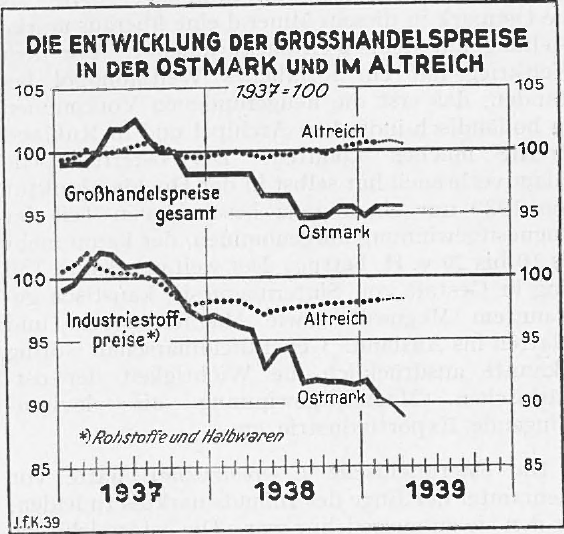
\includegraphics[width=\linewidth]{Experimente/img/f1.png}
        \caption{\hbadness=10000 Liniendiagramm mit komplexer Y-Achse}
        \label{fig:f1}
    \end{minipage}\hfill % Add space between figures
    \begin{minipage}{0.475\textwidth} % Second figure
        \centering
        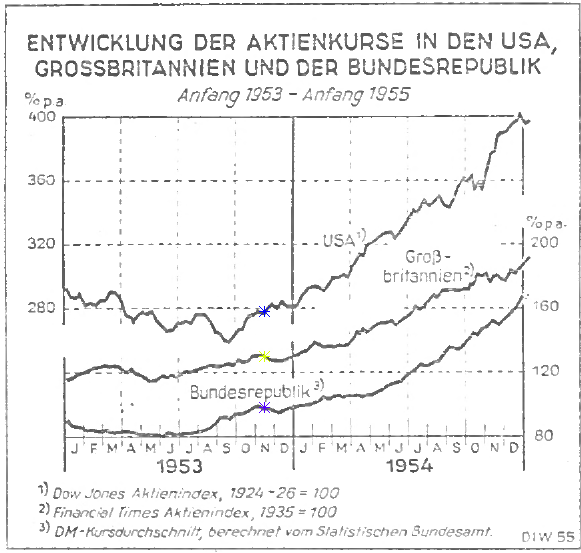
\includegraphics[width=\linewidth]{Experimente/img/f2.png}
        \caption{\hbadness=10000 Liniendiagramm mit unüblicher X-Achse}
        \label{fig:f2}
    \end{minipage}
\end{figure}

Fehlergründe lagen hier bei vereinzelt vorkommenden Lücken in der Werteliniensegmentation, aber der Großteil war dem Achsenerkennungsalgorithmus verschuldet. Abbildungen \ref{fig:f1} und \ref{fig:f2} zeigen Beispiele von zu Fehler führenden Diagrammen. Bei \ref{fig:f1} wird die Y-Achse nach Erreichen des Werts 100 auf 95 zurückgesetzt, um zwei weitere Wertelinien einzubringen, welches Fehler in der linearen Y-Wert-Interpolation hervorruft. Bei \ref{fig:f2} dagegen schlägt die Erkennung der X-Achse fehl, da diese sich unüblicherweise nicht mehr im unteren Rand des Bildes befindet.